\begin{figure}[H]
  \centering
  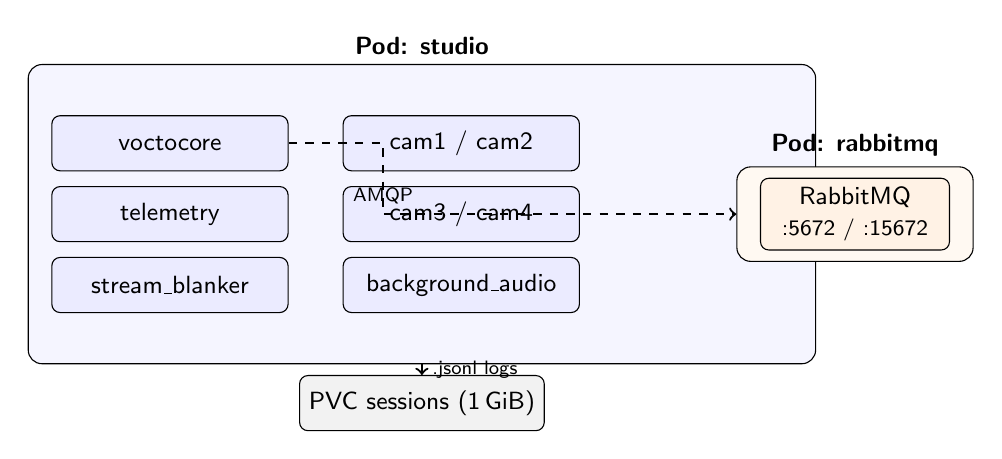
\begin{tikzpicture}[font=\sffamily\small,
    pod/.style={draw, rounded corners=3pt, fill=blue!8,
                minimum width=3.0cm, minimum height=0.7cm, align=center},
    svc/.style={draw, rounded corners=3pt, fill=orange!10,
                minimum width=2.4cm, minimum height=0.7cm, align=center},
  ]
    % Pod studio (multi-contenedor)
    \node[draw, rounded corners=5pt, fill=blue!4, minimum width=10cm,
          minimum height=3.8cm,
          label={[font=\sffamily\bfseries\small]above:Pod: studio}] (studio) at (0,0) {};
    \node[pod] (vc)  at (-3.2, 0.9) {voctocore};
    \node[pod] at (-3.2,-0.0) {telemetry};
    \node[pod] at (-3.2,-0.9) {stream\_blanker};
    \node[pod] at ( 0.5, 0.9) {cam1 / cam2};
    \node[pod] at ( 0.5,-0.0) {cam3 / cam4};
    \node[pod] at ( 0.5,-0.9) {background\_audio};

    % Pod rabbitmq
    \node[draw, rounded corners=5pt, fill=orange!5, minimum width=3.0cm,
          minimum height=1.2cm,
          label={[font=\sffamily\bfseries\small]above:Pod: rabbitmq}]
          (rmq) at (5.5,0) {};
    \node[svc] at (5.5,0) {RabbitMQ\\{\footnotesize :5672 / :15672}};

    % flechas
    \draw[->, thick, dashed] (vc.east) -- ++(1.2,0) |- (rmq.west)
      node[midway, above, font=\sffamily\scriptsize] {AMQP};

    % PVC
    \node[draw, rounded corners=3pt, fill=gray!10, minimum width=2.4cm,
          minimum height=0.7cm, align=center] (pvc) at (0,-2.4)
      {PVC sessions (1\,GiB)};
    \draw[->, thick] (studio.south) -- (pvc.north)
      node[midway, right, font=\sffamily\scriptsize] {.jsonl logs};
  \end{tikzpicture}
  \caption{Arquitectura de pods en el despliegue Kubernetes: el pod \texttt{studio}
           agrupa todos los contenedores del pipeline en un namespace de red compartido;
           \texttt{rabbitmq} corre como pod independiente; el PVC persiste los registros
           de sesión.}
  \label{fig:k8s_pods}
\end{figure}